% Options for packages loaded elsewhere
\PassOptionsToPackage{unicode}{hyperref}
\PassOptionsToPackage{hyphens}{url}
%
\documentclass[
  english,
  man,floatsintext]{apa6}
\usepackage{lmodern}
\usepackage{amssymb,amsmath}
\usepackage{ifxetex,ifluatex}
\ifnum 0\ifxetex 1\fi\ifluatex 1\fi=0 % if pdftex
  \usepackage[T1]{fontenc}
  \usepackage[utf8]{inputenc}
  \usepackage{textcomp} % provide euro and other symbols
\else % if luatex or xetex
  \usepackage{unicode-math}
  \defaultfontfeatures{Scale=MatchLowercase}
  \defaultfontfeatures[\rmfamily]{Ligatures=TeX,Scale=1}
\fi
% Use upquote if available, for straight quotes in verbatim environments
\IfFileExists{upquote.sty}{\usepackage{upquote}}{}
\IfFileExists{microtype.sty}{% use microtype if available
  \usepackage[]{microtype}
  \UseMicrotypeSet[protrusion]{basicmath} % disable protrusion for tt fonts
}{}
\makeatletter
\@ifundefined{KOMAClassName}{% if non-KOMA class
  \IfFileExists{parskip.sty}{%
    \usepackage{parskip}
  }{% else
    \setlength{\parindent}{0pt}
    \setlength{\parskip}{6pt plus 2pt minus 1pt}}
}{% if KOMA class
  \KOMAoptions{parskip=half}}
\makeatother
\usepackage{xcolor}
\IfFileExists{xurl.sty}{\usepackage{xurl}}{} % add URL line breaks if available
\IfFileExists{bookmark.sty}{\usepackage{bookmark}}{\usepackage{hyperref}}
\hypersetup{
  pdftitle={Re-analysing the data from Moffatt et al.~(2020): A textbook illustration of the fallacy of the null hypothesis},
  pdflang={en-EN},
  pdfkeywords={NHST, Bayesian, fallacy, reanalysis, inner speech, rumination, electromyography},
  hidelinks,
  pdfcreator={LaTeX via pandoc}}
\urlstyle{same} % disable monospaced font for URLs
\usepackage{graphicx}
\makeatletter
\def\maxwidth{\ifdim\Gin@nat@width>\linewidth\linewidth\else\Gin@nat@width\fi}
\def\maxheight{\ifdim\Gin@nat@height>\textheight\textheight\else\Gin@nat@height\fi}
\makeatother
% Scale images if necessary, so that they will not overflow the page
% margins by default, and it is still possible to overwrite the defaults
% using explicit options in \includegraphics[width, height, ...]{}
\setkeys{Gin}{width=\maxwidth,height=\maxheight,keepaspectratio}
% Set default figure placement to htbp
\makeatletter
\def\fps@figure{htbp}
\makeatother
\setlength{\emergencystretch}{3em} % prevent overfull lines
\providecommand{\tightlist}{%
  \setlength{\itemsep}{0pt}\setlength{\parskip}{0pt}}
\setcounter{secnumdepth}{-\maxdimen} % remove section numbering
% Make \paragraph and \subparagraph free-standing
\ifx\paragraph\undefined\else
  \let\oldparagraph\paragraph
  \renewcommand{\paragraph}[1]{\oldparagraph{#1}\mbox{}}
\fi
\ifx\subparagraph\undefined\else
  \let\oldsubparagraph\subparagraph
  \renewcommand{\subparagraph}[1]{\oldsubparagraph{#1}\mbox{}}
\fi
% Manuscript styling
\usepackage{upgreek}
\captionsetup{font=singlespacing,justification=justified}

% Table formatting
\usepackage{longtable}
\usepackage{lscape}
% \usepackage[counterclockwise]{rotating}   % Landscape page setup for large tables
\usepackage{multirow}		% Table styling
\usepackage{tabularx}		% Control Column width
\usepackage[flushleft]{threeparttable}	% Allows for three part tables with a specified notes section
\usepackage{threeparttablex}            % Lets threeparttable work with longtable

% Create new environments so endfloat can handle them
% \newenvironment{ltable}
%   {\begin{landscape}\begin{center}\begin{threeparttable}}
%   {\end{threeparttable}\end{center}\end{landscape}}
\newenvironment{lltable}{\begin{landscape}\begin{center}\begin{ThreePartTable}}{\end{ThreePartTable}\end{center}\end{landscape}}

% Enables adjusting longtable caption width to table width
% Solution found at http://golatex.de/longtable-mit-caption-so-breit-wie-die-tabelle-t15767.html
\makeatletter
\newcommand\LastLTentrywidth{1em}
\newlength\longtablewidth
\setlength{\longtablewidth}{1in}
\newcommand{\getlongtablewidth}{\begingroup \ifcsname LT@\roman{LT@tables}\endcsname \global\longtablewidth=0pt \renewcommand{\LT@entry}[2]{\global\advance\longtablewidth by ##2\relax\gdef\LastLTentrywidth{##2}}\@nameuse{LT@\roman{LT@tables}} \fi \endgroup}

% \setlength{\parindent}{0.5in}
% \setlength{\parskip}{0pt plus 0pt minus 0pt}

% \usepackage{etoolbox}
\makeatletter
\patchcmd{\HyOrg@maketitle}
  {\section{\normalfont\normalsize\abstractname}}
  {\section*{\normalfont\normalsize\abstractname}}
  {}{\typeout{Failed to patch abstract.}}
\makeatother
\shorttitle{The fallacy of the null}
\author{Ladislas Nalborczyk\textsuperscript{1}}
\affiliation{
\vspace{0.5cm}
\textsuperscript{1} Univ. Grenoble Alpes, CNRS, Grenoble INP, GIPSA-lab, 38000 Grenoble, France}
\authornote{

Correspondence concerning this article should be addressed to Ladislas Nalborczyk, GIPSA-lab, CNRS, Univ. Grenoble Alpes, 11 Rue des Mathématiques, 38400 Saint-Martin-d'Hères, France. E-mail: ladislas.nalborczyk@gipsa-lab.fr}
\keywords{NHST, Bayesian, fallacy, reanalysis, inner speech, rumination, electromyography}
\usepackage{lineno}

\linenumbers
\usepackage{csquotes}
\ifxetex
  % Load polyglossia as late as possible: uses bidi with RTL langages (e.g. Hebrew, Arabic)
  \usepackage{polyglossia}
  \setmainlanguage[]{english}
\else
  \usepackage[shorthands=off,main=english]{babel}
\fi
\newlength{\cslhangindent}
\setlength{\cslhangindent}{1.5em}
\newenvironment{cslreferences}%
  {\setlength{\parindent}{0pt}%
  \everypar{\setlength{\hangindent}{\cslhangindent}}\ignorespaces}%
  {\par}

\title{Re-analysing the data from Moffatt et al.~(2020): A textbook illustration of the fallacy of the null hypothesis}

\date{}

\abstract{
Moffatt et al.~(2020) reported the results of an experiment (N = 26 in the final sample) comparing the facial (surface) electromyographic correlates of mental rumination and distraction, following an experimentally induced stressor. Based on an absence of significant difference in the perioral EMG-amplitude between the rumination and distraction conditions, Moffatt et al.~(2020) concluded that (the \emph{self-reported}) inner experience was unrelated to peripheral muscular activity as assessed using surface electromyography. We suggest this conclusion is hasty and based on waggly evidence. Indeed, concluding on the absence of an effect based on a low-powered statistical test is strongly problematic/uninformative. Moreover, there relation between self-reports and physiological measures\ldots{} Although the question Moffatt et al.~(2020) pursued is of interest, and mehods\ldots{} Given these limitations, it is unclear whether the target article really adds to the current knowledge. Complete source code, reproducible analyses, and figures are available at \url{https://github.com/lnalborczyk/inner_experience_EMG}.
}

\begin{document}
\maketitle

Wordcount (excluding abstract, references, tables, and figures): 184

\newpage

\hypertarget{introduction}{%
\section{Introduction}\label{introduction}}

\ldots{}

\hypertarget{some-thoughts-on-the-data}{%
\section{Some thoughts on the data}\label{some-thoughts-on-the-data}}

\begin{figure}[!htb]

{\centering 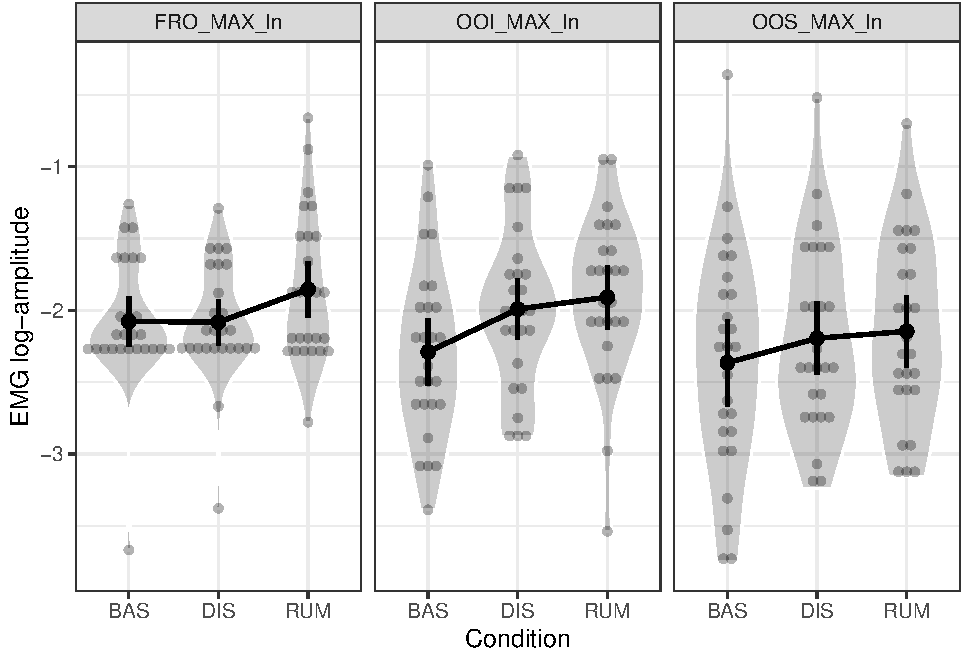
\includegraphics[width=1\linewidth]{reanalysis_files/figure-latex/babar-1} 

}

\caption{General plot (N = 26)...}\label{fig:babar}
\end{figure}

\ldots{}

\hypertarget{concluding-on-the-null-from-low-powered-studies}{%
\subsection{Concluding on the null from low-powered studies}\label{concluding-on-the-null-from-low-powered-studies}}

\url{https://theethicalskeptic.com/2015/08/17/the-four-types-of-null-hypothesis-fallacy/}\ldots{}

Unfortunately, the same line of reasoning applies for testing the effect of the order, which is even less powered than the test of the main effect of interest, rendering it practically uninformative\ldots{}

\begin{quote}
``In order to test this, a Bayesian paired samples t-test was conducted for the peak log values of muscle activity between the rumination and distraction conditions. This revealed strong evidence in favour of the alternative hypothesis for the FRO muscle (B10 = 18.79), and moderate evidence in favour of the null hypothesis for the OOS (B10 = 0.232) and OOI (B10 = 0.278) muscles, according to current guidelines for interpreting Bayes factors {[}43{]}.''
\end{quote}

\ldots{}

\hypertarget{does-everyone}{%
\subsection{Does everyone?}\label{does-everyone}}

\ldots{}

\begin{figure}[!htb]

{\centering 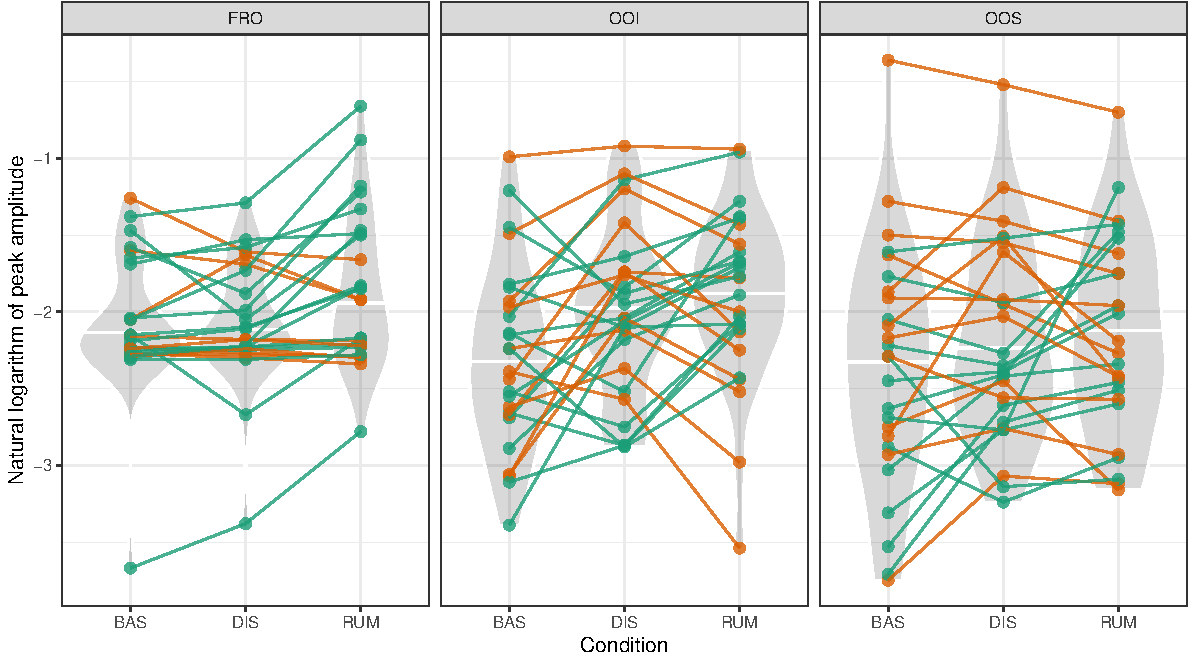
\includegraphics[width=1\linewidth]{reanalysis_files/figure-latex/everyone-1} 

}

\caption{General plot (mean and 95\% CI)... showing the inter-individual variability...}\label{fig:everyone}
\end{figure}

Huge inter-individual variability\ldots{} which leads to the next point, what is the relation between self-reports and EMG?

\hypertarget{relation-between-self-report-and-emg-correlates}{%
\subsection{Relation between self-report and EMG correlates}\label{relation-between-self-report-and-emg-correlates}}

\ldots{}

\hypertarget{discussion-and-conclusions}{%
\section{Discussion and conclusions}\label{discussion-and-conclusions}}

\ldots{}

\hypertarget{supp}{%
\section{Supplementary materials}\label{supp}}

Reproducible code and figures are available at \url{https://github.com/lnalborczyk/inner_experience_EMG}.

\hypertarget{acknowledgements}{%
\section*{Acknowledgements}\label{acknowledgements}}
\addcontentsline{toc}{section}{Acknowledgements}

\ldots{}

\hypertarget{references}{%
\section*{References}\label{references}}
\addcontentsline{toc}{section}{References}

\hypertarget{refs}{}
\begin{cslreferences}
\leavevmode\hypertarget{ref-R-papaja}{}%
Aust, F., \& Barth, M. (2017). \emph{papaja: Create APA manuscripts with R Markdown}. \url{https://github.com/crsh/papaja}

\leavevmode\hypertarget{ref-R-wordcountaddin}{}%
Marwick, B. (2019). \emph{Wordcountaddin: Word counts and readability statistics in r markdown documents}.

\leavevmode\hypertarget{ref-R-here}{}%
Müller, K. (2017). \emph{Here: A simpler way to find your files}. \url{https://CRAN.R-project.org/package=here}

\leavevmode\hypertarget{ref-R-base}{}%
R Core Team. (2017). \emph{R: A language and environment for statistical computing}. R Foundation for Statistical Computing. \url{https://www.R-project.org/}

\leavevmode\hypertarget{ref-R-tidyverse}{}%
Wickham, H. (2017). \emph{Tidyverse: Easily install and load the 'tidyverse'}. \url{https://CRAN.R-project.org/package=tidyverse}

\leavevmode\hypertarget{ref-R-knitr}{}%
Xie, Y. (2015). \emph{Dynamic documents with R and knitr} (2nd ed.). Chapman; Hall/CRC. \url{https://yihui.org/knitr/}

\leavevmode\hypertarget{ref-R-rmarkdown}{}%
Xie, Y., Allaire, J. J., \& Grolemund, G. (2018). \emph{R markdown: The definitive guide}. Chapman; Hall/CRC. \url{https://bookdown.org/yihui/rmarkdown}
\end{cslreferences}

\end{document}
